\section{Logistisches Wachstum}
Das logistische Wachstum stellt einen Wachstumsprozess dar, welcher nicht durchgehend wächst, sondern sich zu einem begrenzten Wachstum wandelt. Ähnlich wie ein begrenztes Wachstum besitzt das logistische Wachstum eine Sättigungsgrenze, die das Wachstum begrenzt. Zu Begin des logistischen Wachstums gilt, dass $f(x)$ proportional zu $f'(x)$ ist. Nach dem Wendepunkt, welcher sich immer bei der Hälfte der Sättigungsgrenze befindet, gilt für $f(x)$, dass es proportional zu der Differenz zu der Sättigungsgrenze ist. Dies bedeutet, dass $S-f(x)$ proportional zu $k(S-f(t))$ ist.
\begin{figure}[h]
	\centering
	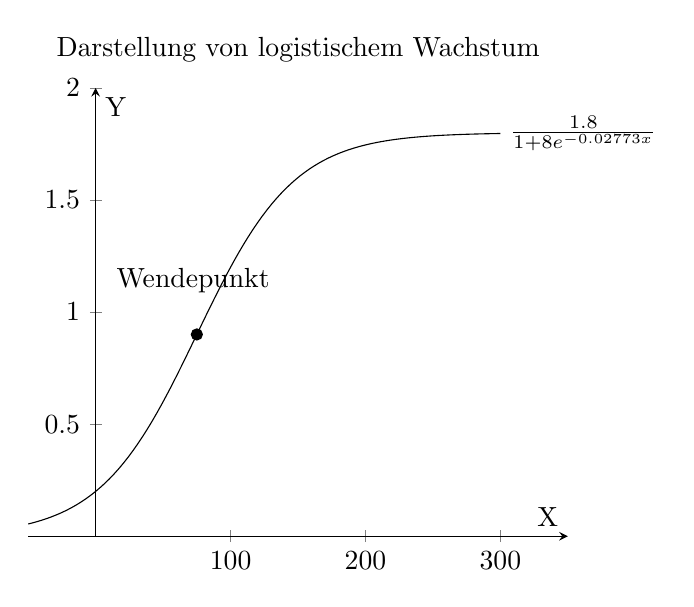
\begin{tikzpicture}
		\begin{axis}[
		title={Darstellung von logistischem Wachstum},
		axis lines=middle,
		clip=false,
		xlabel={X},
		ylabel={Y},
		xmin=-50,
		xmax=350,
		ymin=0,
		ymax=2
		]
		\addplot[domain=-50:300, samples=100]{(1.8)/(1+8*exp(-0.02773*x))} node[right,pos=1]{$\frac{1.8}{1+8e^{-0.02773x}}$};
		\addplot[only marks,mark=*] coordinates {(74.98,0.9)};
        \node[label={above right:{Wendepunkt}}] at (axis cs:1,1) {};
		\end{axis}
	\end{tikzpicture}
	\caption{Der Graph erfüllt bis zu dem Krümmungswechsel die Eigenschaften einer $e$-Funktion, anschließend erfüllt er die Eigenschaften eines Graphen, der ein begrenztes Wachstum darstellt.  }
\end{figure}\\
Das logistische Wachstum wird durch unterschiedliche Normalformen beschrieben. Diese variieren jedoch nur äußerlich. 
	\begin{paracol}{2}
		\[f(t)=\frac{S}{1+\left(\frac{S}{f(0)}\right)e^{-kSt}}\]
		\[f(t)=\frac{f(0)\cdot S}{f(0)+(S-f(0))e^{-kSt}}\]
	\switchcolumn
		\begin{align*}
			f(t)=\frac{f(0)\cdot S\cdot e^{kSt}}{f(0)e^{kSt}+S-f(0)}
		\end{align*}
		\begin{align*}
			f(t)=S-\frac{(S-f(0))S}{f(0)e^{kSt}+S-f(0)}
		\end{align*}
	\end{paracol}
\pagebreak